\section{Benchmarks\label{sec:benchmark}}

\subsection{Benchmarks del proyecto}

Se realizaron pruebas con distintos tipos de tamaño de problemas. Estos tipos de problemas fueron generados a partir de los casos de pruebas utilizados en~\cite{bib:martello00threedimensional}. \\

Dada una superficie de dimensiones $W$ y $H$, se considerarán cinco tipos de items distintos, a saber:

\begin{itemize}
 \item Tipo 1: $w_j$ u.d. en $[1, \frac{1}{2}W]$, $h_j$ u.d. en $[\frac{2}{3}H, H]$, $d_j$ u.d. en $[\frac{2}{3}D, D]$
 \item Tipo 2: $w_j$ u.d. en $[\frac{2}{3}W, W]$, $h_j$ u.d. en $[1, \frac{1}{2}H]$, $d_j$ u.d. en $[\frac{2}{3}D, D]$
 \item Tipo 3: $w_j$ u.d. en $[\frac{2}{3}W, W]$, $h_j$ u.d. en $[\frac{2}{3}H,H]$, $d_j$ u.d. en $[1, \frac{1}{2}D]$
 \item Tipo 4: $w_j$ u.d. en $[\frac{1}{2}W, W]$, $h_j$ u.d. en $[\frac{1}{2}H,H]$, $d_j$ u.d. en $[\frac{1}{2}D,D]$
 \item Tipo 5: $w_j$ u.d. en $[1,\frac{1}{2}W]$, $h_j$ u.d. en $[1,\frac{1}{2}H]$, $d_j$ u.d. en $[1, \frac{1}{2}D]$
\end{itemize}

Para obtener cinco clases de instancias de prueba se considera que para cada clase $k$ ($k=1,\ldots,5$), cada item es de tipo $k$ con una probabilidad de 60\%, y de los otros cuatro tipos con probabilidad de 10\% cada uno. \\

Un segundo grupo de clases se puede obtener de la generalización de las instancias presentadas por Berkey y Wang. Se definen tres clases como sigue:

\begin{itemize}
 \item Clase 6: $W=H=10$, items con $w_j, h_j, d_j$ u.d. en $[1, 10]$.
 \item Clase 7: $W=H=40$, items con $w_j, h_j, d_j$ u.d. en $[1, 35]$.
 \item Clase 8: $W=H=100$, items con $w_j, h_j, d_j$ u.d. en $[1, 100]$.
\end{itemize}

Utilizando estos tipos de items, se procedieron a hacer benchmarks comparando los algoritmos de Branch-and-Bound, provisto por la herramienta ``lp\_solve'' y Enumeración Implicita, programado en C. \\

\begin{table}[!htp]
\centering
\begin{tabular}{||c|l|l|c||}
\hline\hline
Items & B\&B & Enum & Óptimo\\ \hline
3 & 0.007s & 0.003s & Y \\
4 & 0.010s & 0.006s & Y \\
5 & 0.065s & 0.007s & Y \\
6 & 0.594s & 0.011s & Y \\
7 & 1.414s & 0.024s & Y \\
10 & -- & 12.786s & Y \\
14 & -- & 22.010s & Y \\
16 & -- & 35.463s & Y \\ \hline\hline
\end{tabular}
\caption{Benchmarks Branch-and-Bound v/s Enumeración implicita}\label{tabla:07_01}
\end{table}
\pagebreak

\subsection{Benchmarks clásicos}

En la sección describiremos un algoritmo enumerativo para la solución exacta de 3D-SP. Este algoritmo resuelve sub-problema
s asociados repetidamente, en que todos los componentes dados de un subgrupo \(\bar{J}\) tienen que ser situados en un solo
 compartimiento, si es posible. Este problema es NP-duro en el buen sentido, desde la resolución de casos especiales en que
 todos los componentes tienen la misma profundidad $d_j=D$ y el mismo alto $h_j=H$ resolvemos la pregunta si una instancia
del problema Space Planning 2D admite una solución sin necesitar mas que H tableros. En la presente sección describiremos u
n algoritmo \emph{Branco-and-bound} para la solución exacta de una versión optimizada del problema (maximizar el volumen to
tal de los ítems empaquetados), que también es usado en uno de los algoritmos que se describen mas adelante.

El problema que consideraremos es seleccionar un subgrupo \(\bar{J}'\le\bar{J}\) de ítems y asignarles coordenadas \((x_j,
y_j, z_j)\) a cada ítem \(j E \bar{J}\) para que ningún ítem quede afuera del tablero o paquete, no queden traslapados y el
 volumen total de los ítems \(\bar{J}'\) sea un máximo. Para el caso de 2 dimensiones se considera una versión del problema
 de la mochila. Presentaremos una generalización no trivial del caso de 2 dimensiones y daremos un algoritmo efectivo para
este problema. Asumiremos que el origen del sistema de coordenadas esta en la esquina inferior izquierda del tablero.\\
En cada nodo de las ramas del árbol de decisión, que describiremos posteriormente con mayor detalle, una solución parcial q
ue empaqueta los ítems de un subgrupo \(I c \bar{J}\), es incrementado seleccionando y rotando cada ítem \(j E \bar{J}/I\)
y generando nodos descendientes al ubicar j en todos los posibles puntos. Poner un ítem en un punto p significa que su esqu
ina inferior izquierda es posicionada en p.\\

De este modo las coordenadas de p quedan representadas por \((x_j, y_j, z_j)\) : Obviamente el ítem j no puede ser posicion
ado en p si
\(x_p + w_j > W\) o \(y_p + h_j >H\) o \( z_p+d_j >D\). Los puntos que pueden ser considerados se ven reducidos por las sig
uientes propiedades.\\

\emph{Propiedad 1} Cualquier ordenamiento de un tablero puede ser reemplazado por uno equivalente, en que ningún ítem sea m
ovido hacia la izquierda, abajo o atrás.\\
\emph{Propiedad 2} Un Orden óptimo de los ítems existe si \(i < j\), \(X_i + w_i \le x_j\) o \(y_i + h_i \le y_i\) o \(z_i
+ d_i \le z_j\)

\emph{Buscando una posible ubicación para posicionar un ítem} \\

Solucionaremos este problema mediante repeticiones de problemas de 2 dimensiones, considerando las caras x-y como un subcon
junto de los ítems. Así empezaremos con la descripción del algoritmo de dos dimensiones.\\
Dado un ítem I, es fácil encontrar, en dos dimensiones el sistema \emph{C(I)} de puntos de las esquinas que recubre el objeto, asociada a la región factible \emph{S(I)} definida por las caras \emph{x-y} de los ítems en I. Ordenemos los ítems de acuerdo a sus puntos finales \((x_j+w_j,y_j+h_j)\), de modo que los valores \(y_j+h_j\) no se incrementen, rompiendo vínculos con los valores mas grandes de \(x_j+w_j\). El siguiente algoritmo para determinar los puntos de la esquina, consta de tres fases: Primero, ítems extremos son encontrados, i.e., ítems cuyos puntos finales coinciden con un punto en que el entorno cambia de horizontal a vertical. En la segunda fase, puntos de la esquina son definidos como intersecciones entre las líneas que conducen desde puntos finales de ítems extremos. Finalmente esquinas no factibles donde ningún otro ítem \(\bar{J}/I\) pueda entrar, son removidas. Así tenemos el siguiente algoritmo:\\

\begin{figure}[!htb]
\centering
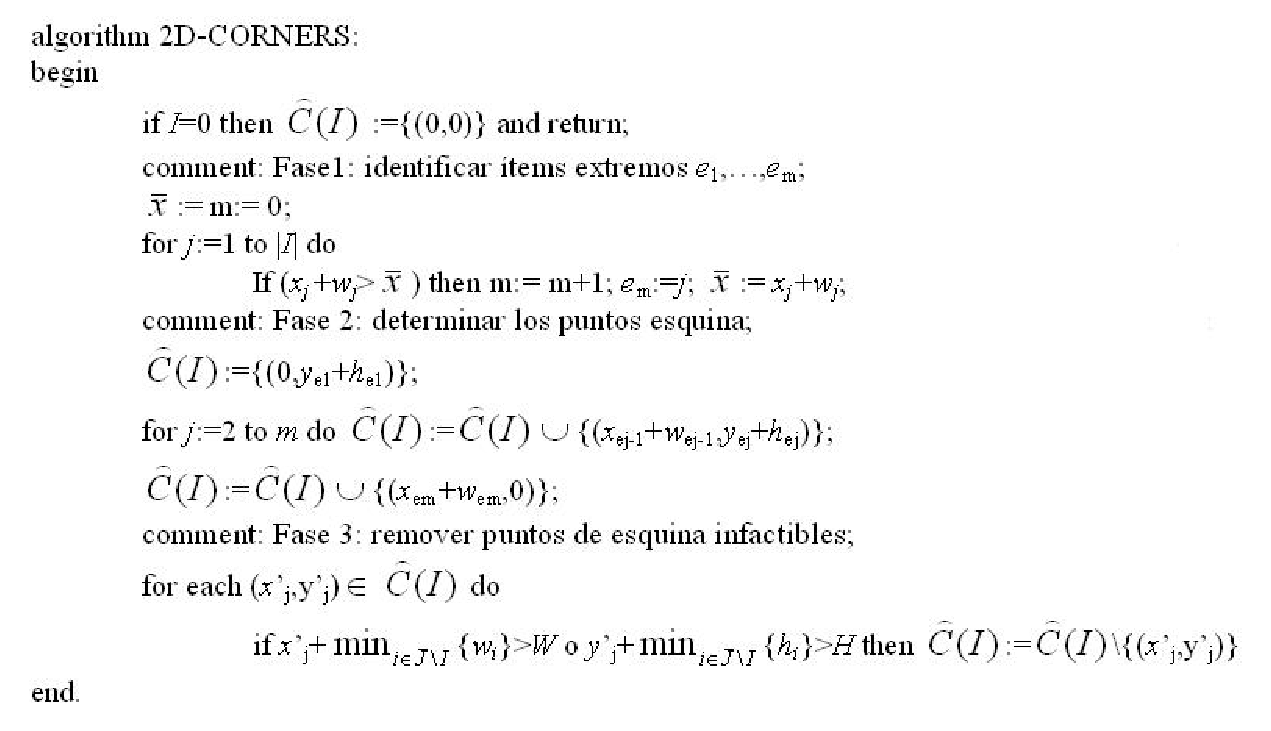
\includegraphics[scale=0.6]{fotos/foto1.eps}
\caption{Algoritmo 2D-CORNERS}
\end{figure}

\begin{figure}[!htb]
\centering
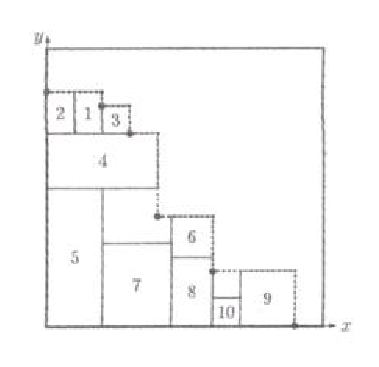
\includegraphics[scale=0.6]{fotos/foto2.eps}
\caption{Envoltura plana del bin}
\end{figure}

Considerando el ejemplo de la figura 2: los ítems extremos 1, 3, 4, 6 y 9 y los puntos de las esquinas resultantes están in
dicados por puntos negros; Fase 3 puede remover algunos de los primeros y/o últimos puntos de las esquinas.\\
La complejidad del 2D-CORNERS es \(O(|I|)\), mas \(O(|I| log |I|)\) para el ordenamiento del ítem inicial, i.e., \(O(n)\) m
as \(O(n log n)\).\\
Asumimos que los puntos de las esquinas resultantes son \(C(I)={(x'_j,y'_j),\dots{},(x'_l,y'_l)}\ne 0\). Entonces el área o
cupada es:

\begin{figure}[!htb]
\centering
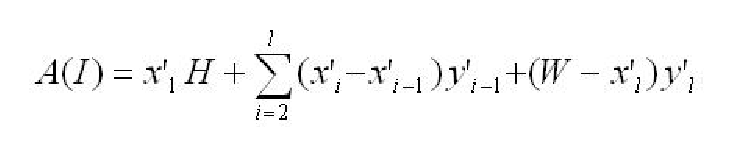
\includegraphics[scale=0.6]{fotos/foto3.eps}
\caption{Área utilizada dentro de la superficie}
\end{figure}

Donde el primero termino es no cero siempre que el punto de la esquina encontrado en la fase 2 sea removido en la fase 3. E
n el caso especial donde \(C(I)=0\), obviamente asignamos \(A(I)=WH\).\\
El algoritmo 2D-CORNERS puede ser usado para determinar el sistema \(C(I)\) de puntos de las esquinas en tres dimensione
s, donde I es el sistema de tres dimensiones actualmente empaquetado dentro del contenedor. Se puede aplicar para z=0 y par
a cada z distinto donde un ítem I termina, mediante incremento de valores. Para tales coordenadas z', 2D-CORNERS puede ser
aplicado a cada subsistema de ítems \(i E I\) que terminan despues de z', es decir:\\

\begin{center}
\(z_i + d_i >z'\)
\end{center}
agregando los puntos de las esquinas resultantes a \(C(I)\). Mediante este camino, uno puede sin embargo obtener algún punt
o falso, desde que son puntos del caso de 2 dimensiones pero no en el caso de 3 dimensiones. Esos puntos son fácilmente rem
ovidos por dominación, donde decimos que el punto \((x'_a,y'_a,z'_a)\) domina a otro punto \((x'_b,y'_b,z'_b)\) que esta es
condido detrás de el. Formalmente esto se escribe así:

\begin{center}
\(x'_a=x'b\) y \( z'_a=y'b\) y \(z'_a < z'_b\)\\
\end{center}
Donde tenemos igualdades en las dos primeras expresiones, asegurando que todos los ítem en frente de \(z'_k\) sean elegidos
 y ahi no se generaran puntos dentro del área. Esto se hace en el siguiente algoritmo, donde la generación de puntos finale
s tan pronto como la coordenada z es encontrada tales ítems no factibles pueden ser posicionados después de el.\\

\begin{figure}[!htb]
\centering
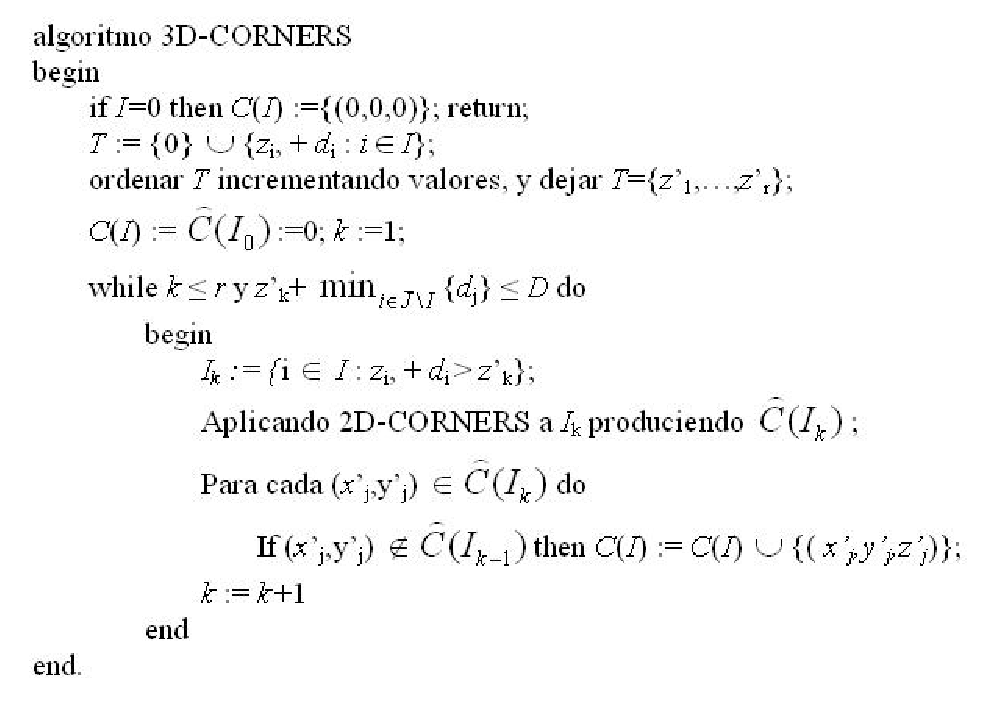
\includegraphics[scale=0.6]{fotos/foto4.eps}
\caption{Algoritmo 3D-CORNERS}
\end{figure}

La complejidad de 3D-CORNERS es \(O(n^2)\) de hecho hay mas coordenadas \(|I|+1\) distintas de  z en  T, y cada sistema \(C(I_k)\) es derivado de 2D-CORNERS en \(O(|I_k|)\), desde que el ordenamiento de ítems puede ser hecho desde el comienzo para los algoritmos. Para cada valor de  \(z'_k\) el chequeo de los puntos requiere \(O(|C(I_k)|)\) en total, desde que ambos \(C(I_k)\) y \(C(I_k)\) son ordenados por incremento de \(x'_j\) y decreciendo \(y'_j\). La complejidad total seguida de la observación de ambas \(|I|\) y \(C(I_k)\) es \(O(n)\).\\

sumiendo que k* es el induce de los I* 3D-CORNERS generados, el volumen V(I) ocupado por los ítems asociado a I es:\\

\begin{figure}[!htb]
\centering
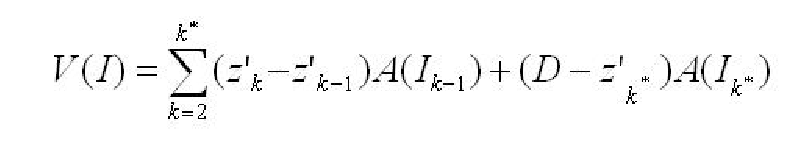
\includegraphics[scale=0.6]{fotos/foto5.eps}
\caption{Volumen utilizado dentro del bin}
\end{figure}

\begin{figure}[!htb]
\centering
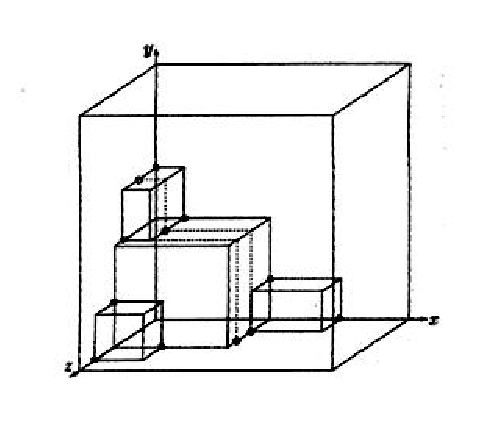
\includegraphics[scale=0.6]{fotos/foto6.eps}
\caption{Envoltura en el espacio 3D}
\end{figure}

\emph{Algoritmos exactos y aproximaciones para 3D-SP.}\\

El algoritmo exacto para 3D-SP esta basado en una descomposición de 2 niveles. Un árbol de ramificaron principal asigna íte
ms a contenedores sin especificar su posición actual, mientras que una versión especializada del algoritmo es usada para lo
s nodos seguros, testeando los sub ítems que pueden ser introducidos dentro de un contenedor simple. Para construir una bue
na solución inicial 2 heurísticas se han definido, una basada en \emph{first-fit-decreasing} y otra basada en la versión \emph{m-cut} del algoritmo ONEBIN\\

\emph{Árbol principal de ramificación}\\

El árbol principal de ramificaciones asigna ítems a los diferentes contenedores especificando su actual posición. Los ítems
 son previamente ordenados de acuerdo a volúmenes decrecientes y la exploración sigue una estrategia de \emph{profundidad-p
rimero}. Sea Z el valor de la solución segura y \(M = {1,\dots{},m}\) el actual sistema de contenedores. Un contenedor de M
 es llamado abierto de otro modo estaría cerrado.\\
En cada nodo de decisión el próximo ítem libre es asignado a todos los contenedores abiertos si \(|M| < Z - 1\) el ítem es
también asignado a un nuevo contenedor.\\
Cuando un ítem k es asignado a un contenedor i que ya contiene un subconjunto, por ejemplo \(\bar{J} \cup k'\). Si el limit
e inferior es mayor que uno para cada k', el contenedor esta cerrado, por lo tanto no se pueden introducir mas ítems en el.
 De otro modo la siguiente regla es testeada. Sea K un subconjunto de los ítems libres que se han generado sobre el limite
inferior. Si una heurística puede encontrar un contenedor para la instancia definida por los ítems en  sabemos que no hay u
na mejor posición posible.\\

\emph{Algoritmos de aproximación}\\

Para obtener una buena cota superior para el nodo raíz del árbol de ramificación y acotar el número de ejecuciones de ONEBIN
, dos diferentes heurísticas son definidas. Dos aproximaciones proveen un complemento computacional. Para desempeños muy ba
jos de una, la otra proporciona desempeños mas elevados, sin embargo la segunda entrega mejores resultados.\\

